\section{Razvoj nove verzije Fibonacci aplikacije}
U drugoj verziji poboljšana je vremenska kompleksnost tako što je uklonjena rekurzija te dodana
memoizacija. Nova vremenska kompleksnost je $O(N)$, dok je memorijska kompleksnost $O(1)$. Nova
verzija prikazana je kodom~\ref{04fibv2}. U novoj je verziji također izmijenjen dizajn kao što je
prikazano slikom~\ref{fig:04redesign}

\lstset{caption={Fibonacci v2}, label=04fibv2}
\begin{lstlisting}[float=h]
func fibonacci(n uint64) uint64 {
	if n == 0 {
		return 0
	}
	a := uint64(0)
	b := uint64(1)

	for n > 1 {
		tmp := a + b
		a = b
		b = tmp
		n--
	}
	return b
}
\end{lstlisting}

\begin{figure}[h]
    \centering
    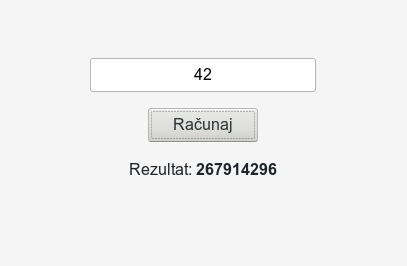
\includegraphics[width=0.5\textwidth]{img/04/new_app.png}
    \caption{Novi dizajn Fibonacci aplikacije}%
    \label{fig:04redesign}
\end{figure}

Nakon što su napravljene izmjene unutar aplikacije, potrebno je spremiti izmjene unutar Git
repositorija te poslati izmjene na servis za pregled koda. Primjer za spremanje izmjena i slanje na
udaljeni Git poslužitelj pomoću komandne linije prikazan je kodom~\ref{04gitreview}.

\lstset{caption={Spremanje i slanje izmjena na Git poslužitelj}, label=04gitreview}
\begin{lstlisting}[float=h]
# nova git grana pod nazivom optimizacija
git checkout -b optimizacija

# dodaj datoteku main.go koja sadrzi izmjene
git add main.go

# dodaj izmjenu
git commit -m "Optimizacija Fibonacci funkcije"

# posalji izmjene na server i prati udaljenu granu
git push -u origin optimizacija
\end{lstlisting}

Kada je kod pregledan i odobren tada se prebacuje u \textit{master} granu. Sustavi za reviziju koda
u pravilu to automatski odrađuju nakon što je kod potvrđen za spajanje. Ručno prebacivanje prikazano
je kodom~\ref{04gitmerge}.

\lstset{caption={Spremanje i slanje izmjena na Git poslužitelj}, label=04gitmerge}
\begin{lstlisting}[float=h]
# prelazak u master git granu
git checkout master

# spajanje grane optimizacija u granu master
git merge optimizacija

# posalji izmjene na server, master grana
git push origin master
\end{lstlisting}

Jenkins pokreće izgradnju nove aplikacije čim je nekakva izmjena dostupna na Git poslužitelju unutar
glavne, \textit{master} grane. Ukoliko su svi testovi uspješni objavljuje se Docker slika. Zatim
servis za menadžment dohvaća novu verziju te počinje posluživati korisnike s novom verzijom.

Prethodnu verziju aplikacije potrebno je ukloniti tek nakon što su svi zahtjevi obrađeni. Na
primjer, ukoliko je potrebno dvije sekunde za obradu nekog zahtjeva, tada je potrebno pričekati
barem toliko vremena prije nego što se prethodna verzija aplikacije može potpuno ugasiti.  U
protivnom zahtjev korisnika će biti prekinut i neće biti potpuno ispunjen.

Testiranje stabilnosti aplikacije prilikom izmjene koda provedeno je alatom \textit{Jmeter}. Jmeter
je alat za stresno testiranje aplikacije, a razvija ga neprofitna organizacija \textit{Apache}. Može
se koristiti za stresno testiranje FTP, LDAP, HTTP, baza podataka preko JDBC, i mnogih drugih
protokola.

Za testiranje infrastrukture ovog projekta korišten je HTTP protokol. Izvršeno je 10.000 zahtjeva
za 34.~Fibonaccijev broj. U trenutku pokretanja stresnog testa korištena je stara verzija Fibonacci
aplikacije, a potom je objavljena nova verzija koja sadrži optimizaciju. Svi zahtjevi uspješno su
izvršeni. Na slici~\ref{fig:04stresstest} prikazan je vremenski odaziv prve i druge verzije
aplikacije.

\begin{figure}[h]
    \centering
    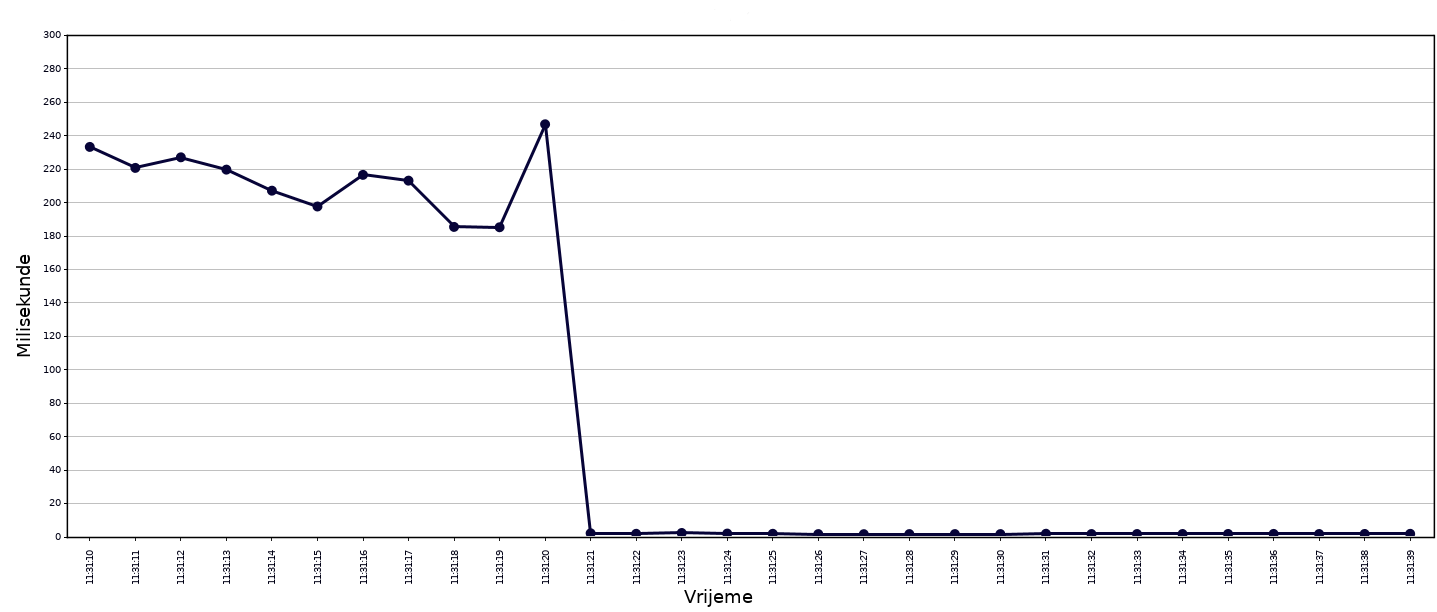
\includegraphics[width=\textwidth]{img/04/response_time.png}
    \caption{Vrijeme odaziva aplikacije}%
    \label{fig:04stresstest}
\end{figure}

\section{Tipični problemi s objavom nove verzije aplikacije}
Bilo koja izmjena aplikacije može uzrokovati neočekivanu pogrešku, stoga svaka izmjena aplikacije
predstavlja rizik. Osim logičkih grešaka unutar aplikacije, koje se mogu otkriti testovima jedinice
i \textit{end-to-end} testovima, moguće se i greške koje se događaju samo prilikom objavljivanja
nove verzije. Primjerice, aplikacija može zapisivati podatke unutar baze podataka u određenom
formatu koji nije kompatibilan s novom verzijom aplikacije. Vraćanje na prethodnu verziju aplikacija
može dovesti i do dodatnih komplikacija ukoliko korisnik u trenutku ima novu verziju s novom bazom
podataka.

Tipični problemi s objavom nove verzije aplikacija su:
\begin{itemize}
    \item nekompatibilnost privremene memorije (\textit{engl. cache})
    \item nekompatibilnost baze podataka
    \item nekompatibilnost programskog sučelja klijenta i poslužitelja
\end{itemize}

Nekompatibilnost privremene memorije javlja se kada nova verzija aplikacije promjeni strukturu
privremene memorije te očita neočekivan podatak generiran iz prijašnje verzije aplikacije. Situacija
se može dodatno zakomplicirati ako su u danom trenutku pokrenute dvije verzije. Kako bi se izbjegla
takva situacija najčešće se preporuča novi ključ za privremenu memoriju ili progresivna izmjena
podataka privremene memorije. Prilikom korištenjem novog ključa nova aplikacija piše u novu
privremenu memoriju te ne ovisi o prethodnoj verziji. Ovakvo rješenje ima problem s hladnom
predmemorijom (\textit{engl. cold cache}) koje uzrokuje s povećanim vremenom odaziva. Druga opcija
je progresivna izmjena podataka koja zahtjeva dodatni kod kako bi stari i novi unos bio kompatibilan
s obje verzije aplikacije. Potrebne su barem dvije verzije i neko vrijeme kako bi se mogla ispustiti
podrška za prethodnu strukturu predmemorije.

Na primjeru Fibonacci aplikacije, zamislimo da koristimo sustav za memoriju, kao na primjer
\textit{memcached}. U trenutnoj verziji aplikacija sprema vrijednost N-tog Fibonaccijev broja pod
ključem \textit{fibonacci-N}. U trenutnoj verziji aplikacije odlučeno je da je prvi Fibonaccijev
broj nula, a drugi broj jedan. No u novoj verziji aplikacije odlučeno je koristiti originalnu
verziju algoritma, tako da su i prvi i drugi Fibonaccijevi brojevi jednaki broju jedan. Ukoliko se
rezultati memorije ne uklone ili spreme pod drugim ključem, tada će nova verzija Fibonacci
aplikacije i dalje vraćati stare rezultate.

Nekompatibilnost baze podataka je slična nekompatibilnosti privremene memorije. No za razliku od
privremene memorije, nije moguće izabrati novi ključ jer u tom slučaju stari podaci neće biti
dostupni korisniku. Inženjer može izabrati migraciju sa stankom aplikacije ili bez stanke. Migracija
sa stankom aplikacije je u pravilu jednostavnija izvedba. No, takva stanka je negativno korisničko
iskustvo. Firme poput Google i Facebook uvijek koriste migracije bez stanke. Kako bi se migracija
mogla napraviti bez stanke potrebno je nekoliko faza i verzija aplikacija. Često se takva migracija
svodi na:
\begin{itemize}
    \item izmjene sheme baze podataka, ali takve izmjene da su kompatibilne sa prethodnom verzijom
        aplikacije
    \item izmjene aplikacije koja omogućava zapis u izmijenjenu bazu podataka bez da utječe na
        prethodnu verziju aplikacije
    \item prijepis povijesnih podataka u novu shemu (\textit{engl. backfill})
    \item izmjene aplikacije tako da se ne zapisuju podaci u staru shemu baze podataka
    \item izmjene sheme baze podataka gdje se stare vrijednosti uništavaju.
\end{itemize}

Kod nekompatibilnosti programskog sučelja klijenta i poslužitelja dolazi prilikom objave nove
aplikacije i promjenom sučelja na poslužitelju, to jest aplikaciji. Slika \ref{fig:04request_flow}
prikazuje pojednostavljeni primjer korisničke interakcije s Fibonacci aplikacijom prilikom objave
nove verzije aplikacije.

\begin{figure}[h]
    \centering
    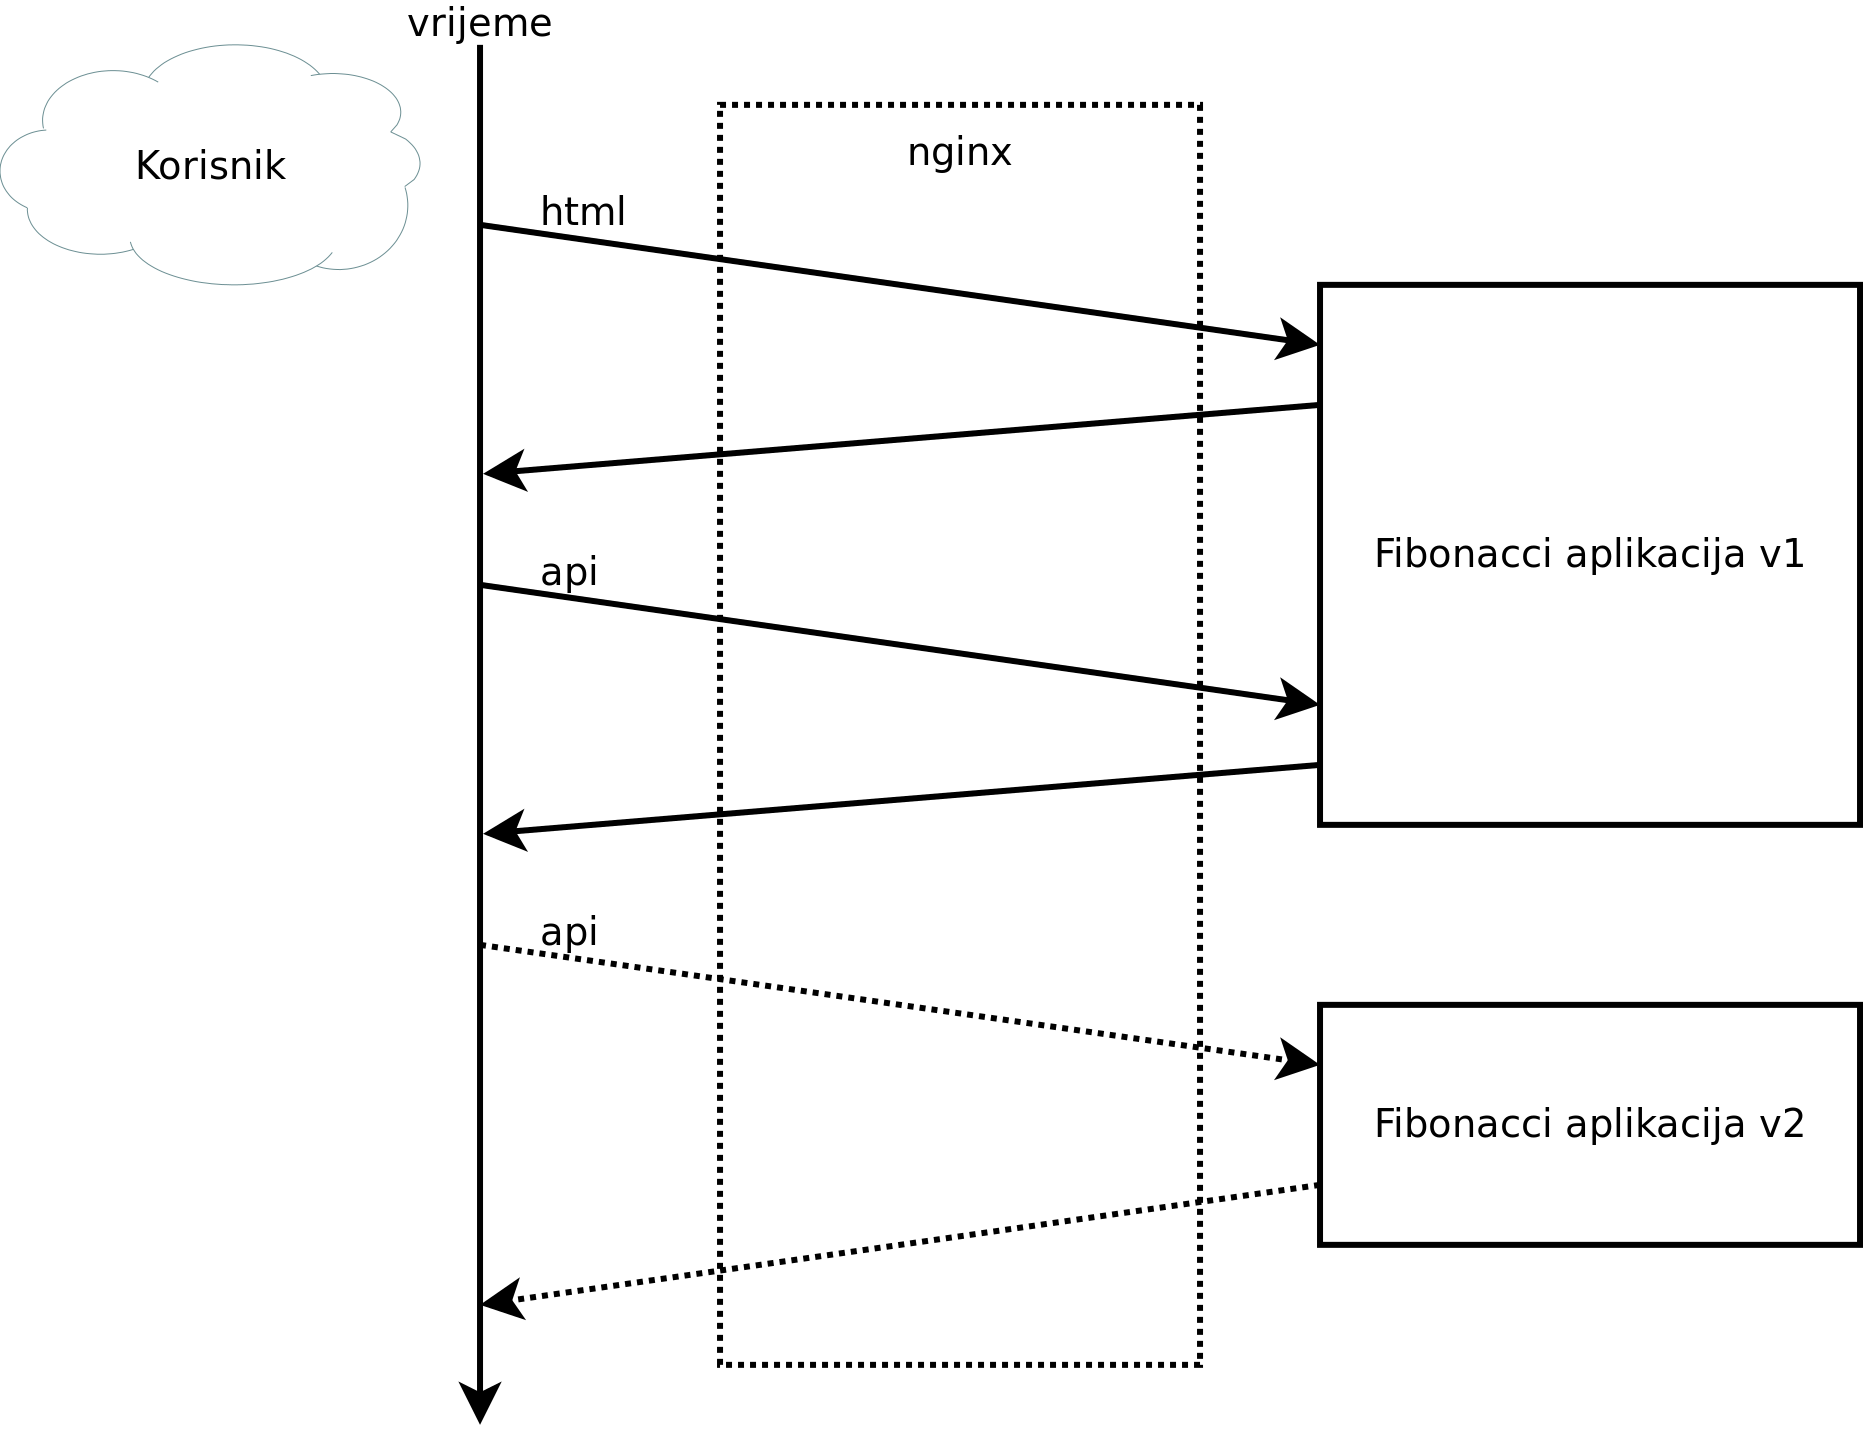
\includegraphics[width=\textwidth]{img/04/request_flow.png}
    \caption{Objava nove verzije aplikacije}%
    \label{fig:04request_flow}
\end{figure}

Korisnik prvo zahtjeva početnu HTML stranicu koja sadrži formu i klijentski Javascript kod koji
određuje gdje će se zahtjev poslati nakon što korisnik upiše broj i pritisne gumb "Računaj". Na
slici, prvi zahtjev je prema aplikacijskom sučelju (API) originalne verzije. No, drugi zahtjev
upućen je novoj verziji aplikacije. Ukoliko nova verzija ima drugačije sučelje, takav zahtjev neće
uspjeti te će korisniku biti poslana greška. Jedini način da web aplikacija ponovno proradi je tako
da korisnik ručno osvježi (\textit{engl. refresh}) web stranicu, što je negativno korisničko
iskustvo.

Kako bi se to izbjeglo, potrebno je zadržati kompatibilnost programskog sučelja trenutne i nove
verzije aplikacije. Nakon određenog vremena se može očekivati da će korisnici imati novu klijentsku
verziju aplikacije te se kompatibilnost može maknuti. U praksi se zna i pitati korisnika za
osvježavanje stranice.

\section{Vraćanje na staru aplikaciju}
Kao što je rečeno u prethodnom poglavlju, svaka izmjena aplikacije može uzrokovati s neočekivanom
pogreškom. Korištenjem testova jedinica i \textit{end-to-end} testova povećana je vjerojatnost
otkrivanja greške prilikom razvoja aplikacije. No, ukoliko novoobjavljena verzija aplikacije sadrži
neku grešku, potreban je dobar sustav kako bi se takva pogreška mogla brzo otkloniti. Često je
najbrže rješenje vraćanje na staru verziju aplikacije (\textit{engl.~version rollback}), gdje se
neispravna verzija zamjenjuje s prethodno objavljenom, stabilnom verzijom. Zatim je potrebno
ukloniti grešku u kodu te dodati prikladne testove nakon čega se može objaviti nova, ispravljena
verzija aplikacije.

Proces vraćanja na staru verziju mora biti brz i intuitivan. U ovom radu korišten je
parametrizitrani Jenkins posao za vraćanje na prethodno objavljenu verziju, prikazan
slikom~\ref{fig:04jenkins_rollback} i kodom~\ref{04:jenkins_revert}. Prilikom pokretanja takvog
posla korisniku je dan padajući izbornik sa svim verzijama aplikacije. Nakon što korisnik izabere
željenu verziju, Jenkins označava tu verziju aplikacije kao zadnju. Unutar trideset sekundi servis
za menadžment pokreće novoizabranu verziju aplikacije i počinje ju posluživati. U tom trenutku
verzija aplikacije s greškom se više ne poslužuje korisnicima.

\begin{figure}[h]
    \centering
    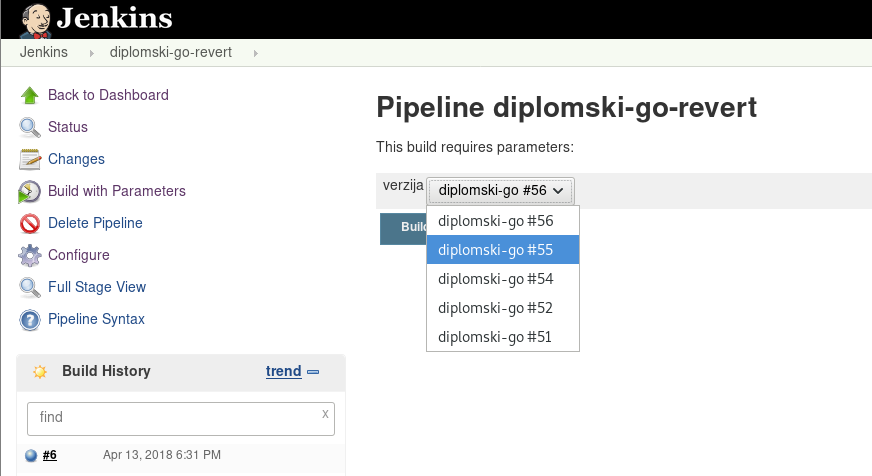
\includegraphics[width=\textwidth]{img/04/jenkins_rollback.png}
    \caption{Jenkins posao za vraćanje verzije aplikacije}%
    \label{fig:04jenkins_rollback}
\end{figure}

\lstset{caption={\textit{Jenkinsfile} za vraćanje na prethodnu verziju}, label=04:jenkins_revert}
\begin{lstlisting}[float=h]
pipeline {
    agent any
    stages {
        stage('Objava slike') {
            steps {
                script {
                    docker.withRegistry('https://docker.io', 'dockerhub') {
                        def i = docker.image("sokac/fibonacci:${VERZIJA_NUMBER}")
                        i.push('latest')
                    }
                }
            }
        }
    }
}
\end{lstlisting}
